\chapter{Data and MC samples}
\label{ch:ana-intro}

\section{Data samples}

\par The proton-proton collisions at a centre-of-mass energy of 13~TeV recorded between 2015 and 2017 are used in this search, and the corresponding good-run-lists are showed below:

\begin{itemize}
	\scriptsize
	\item \texttt{data15\_13TeV.periodAllYear\_DetStatus-v89-pro21-02\_Unknown\_PHYS\_StandardGRL\_All\_Good\_25ns.xml}
	\item \texttt{data16\_13TeV.periodAllYear\_DetStatus-v89-pro21-01\_DQDefects-00-02-04\_PHYS\_StandardGRL\_All\_Good\_25ns.xml}
	\item \texttt{data17\_13TeV.periodAllYear\_DetStatus-v99-pro22-01\_Unknown\_PHYS\_StandardGRL\_All\_Good\_25ns\_Triggerno17e33prim.xml}
	\item \texttt{data18\_13TeV.periodAllYear\_DetStatus-v102-pro22-04\_Unknown\_PHYS\_StandardGRL\_All\_Good\_25ns\_Triggerno17e33prim.xml}
\end{itemize}

\par The resulting dataset corresponds to integrated luminosities of 3.2~\ifb, 33.0~\ifb, 44.3~\ifb\ and 58.5~\ifb\ for each data taking year, respectively. 
The total integrated luminosity is 139.0~\ifb.

\section{Trigger}
\label{sec:trigger}

\par \MET~triggers is used in 0 and 1 lepton regions and unprescaled single-muon triggers in the 2 lepton region. 
Their thresholds are determined by requiring lowest unprescaled single-muon triggers~\cite{lowest_unprescaled_triggers}. 

\par An offline cut \MET~$>$ 150~GeV is applied as the triggers are not fully efficient in low \MET~region. Since the trigger turn-on curve is not well modeled in MC,
 trigger efficiencies are measured in both data and MC from a single-muon measurement region, and scale factors are calculated to correct
turn-ons in MC to match data in the signal region and the single-muon control region.

\par \METnomu~compensates the online \MET~which is reconstructed using only calorimeter informationin without the contribution of the muon.
Events collected with the muon trigger can be used to measure the trigger turn-on curve of the \MET~trigger. 

\par The efficiencies of \MET~triggers are derived in a single-muon measurement region.
The event selection is same as the selection in the resolved regime in Chapter~\ref{ch:ana-sig}, except for the cut on \met.
The efficiencies are calculated inclusively in the number $b$-jets to allows for a larger statistics in the measurement region.

\par The \MET~trigger efficiency is defined by:

\begin{equation}
	\label{eq:trigeff}
	\text{efficiency} = \frac{\text{\#Events passed selection AND \MET~trigger requirement}}{\text{\#Events passed selection}}
\end{equation}

\par The efficiencies are calculated for each \MET~trigger separately within the data-taking periods in which it was used, and separately for data and MC.
 The trigger efficiency curves for each \MET~trigger are shown in Fig.~\ref{fig:TrigEff} as a function of \METnomu~to mimic the \MET~topology on trigger level.

\begin{figure}[tb!]
	\centering
	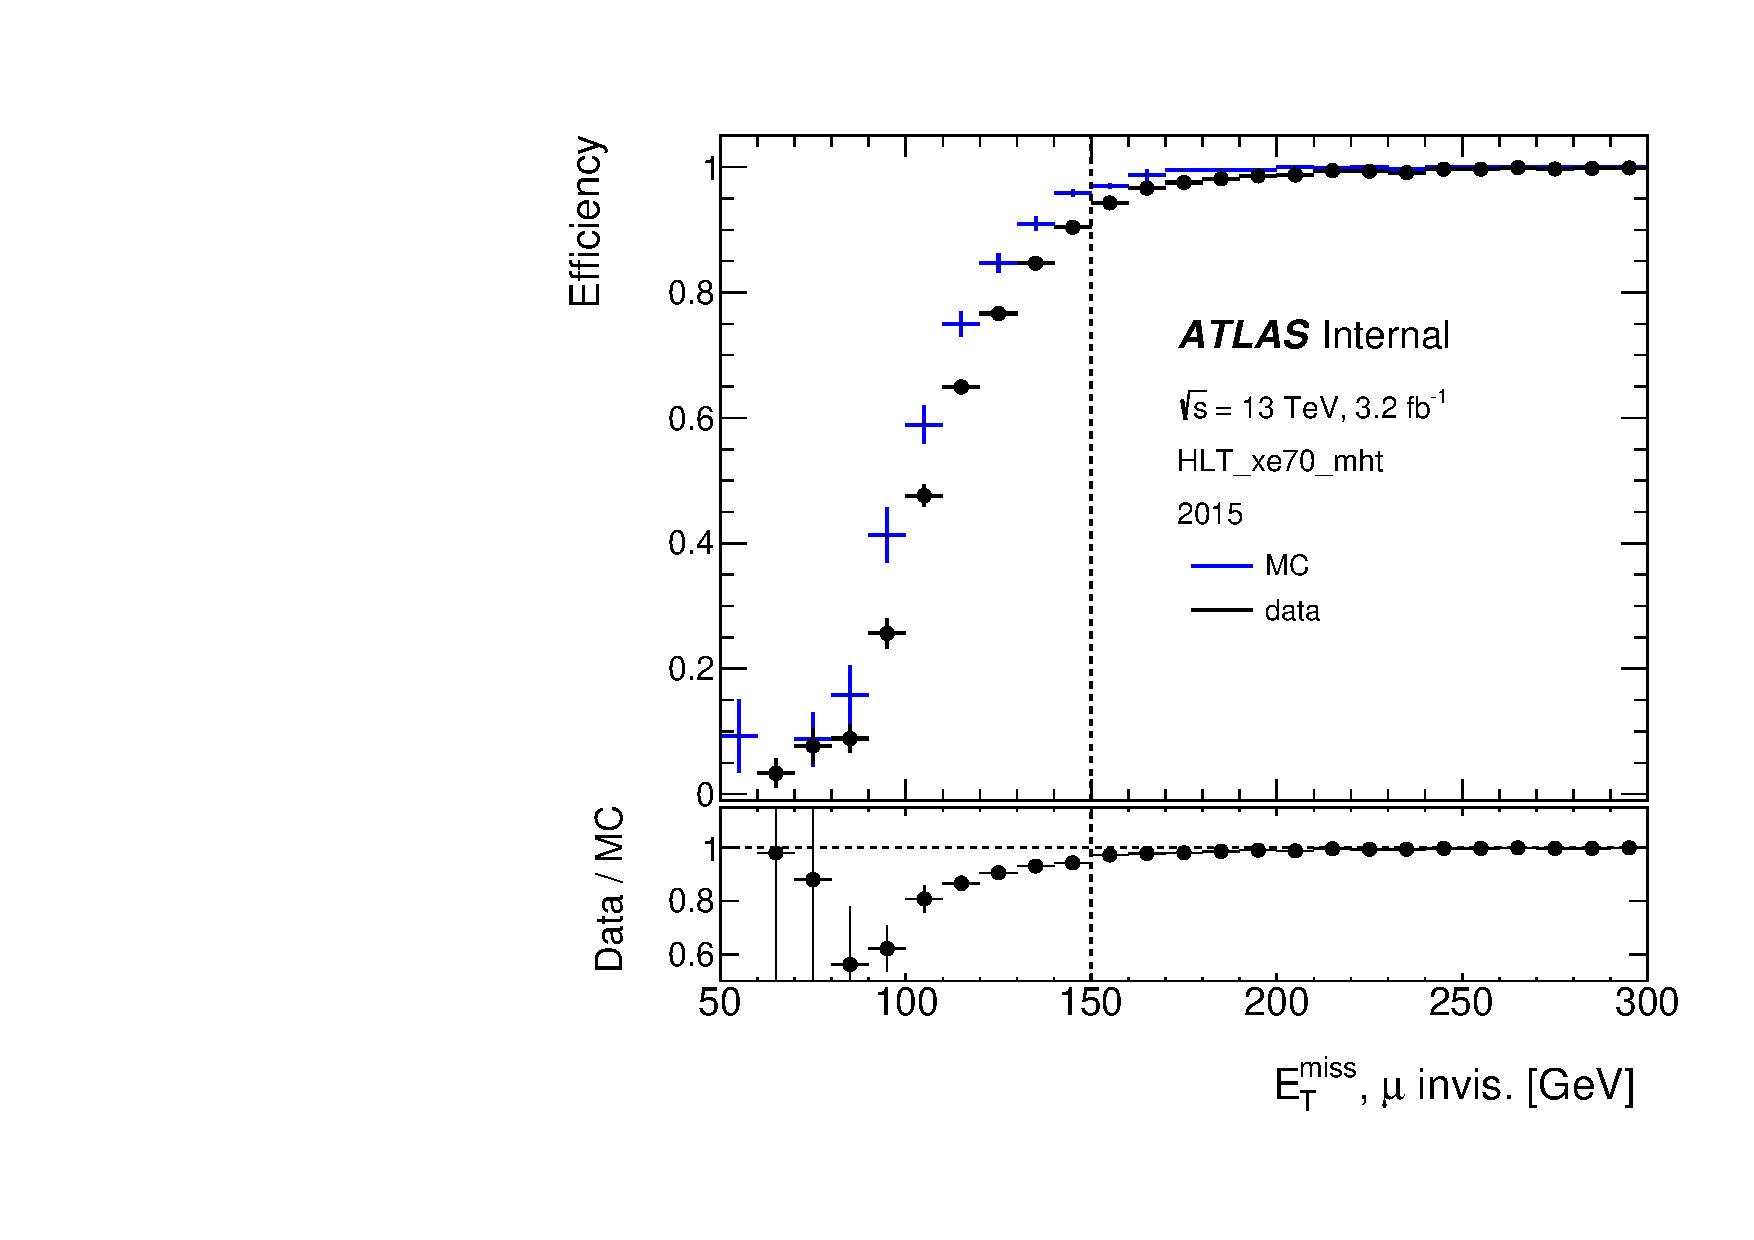
\includegraphics[width=0.45\textwidth]{chapters/c6/figures/METTriggerCalibration/efficiecy_HLT_xe70_mht.pdf}
	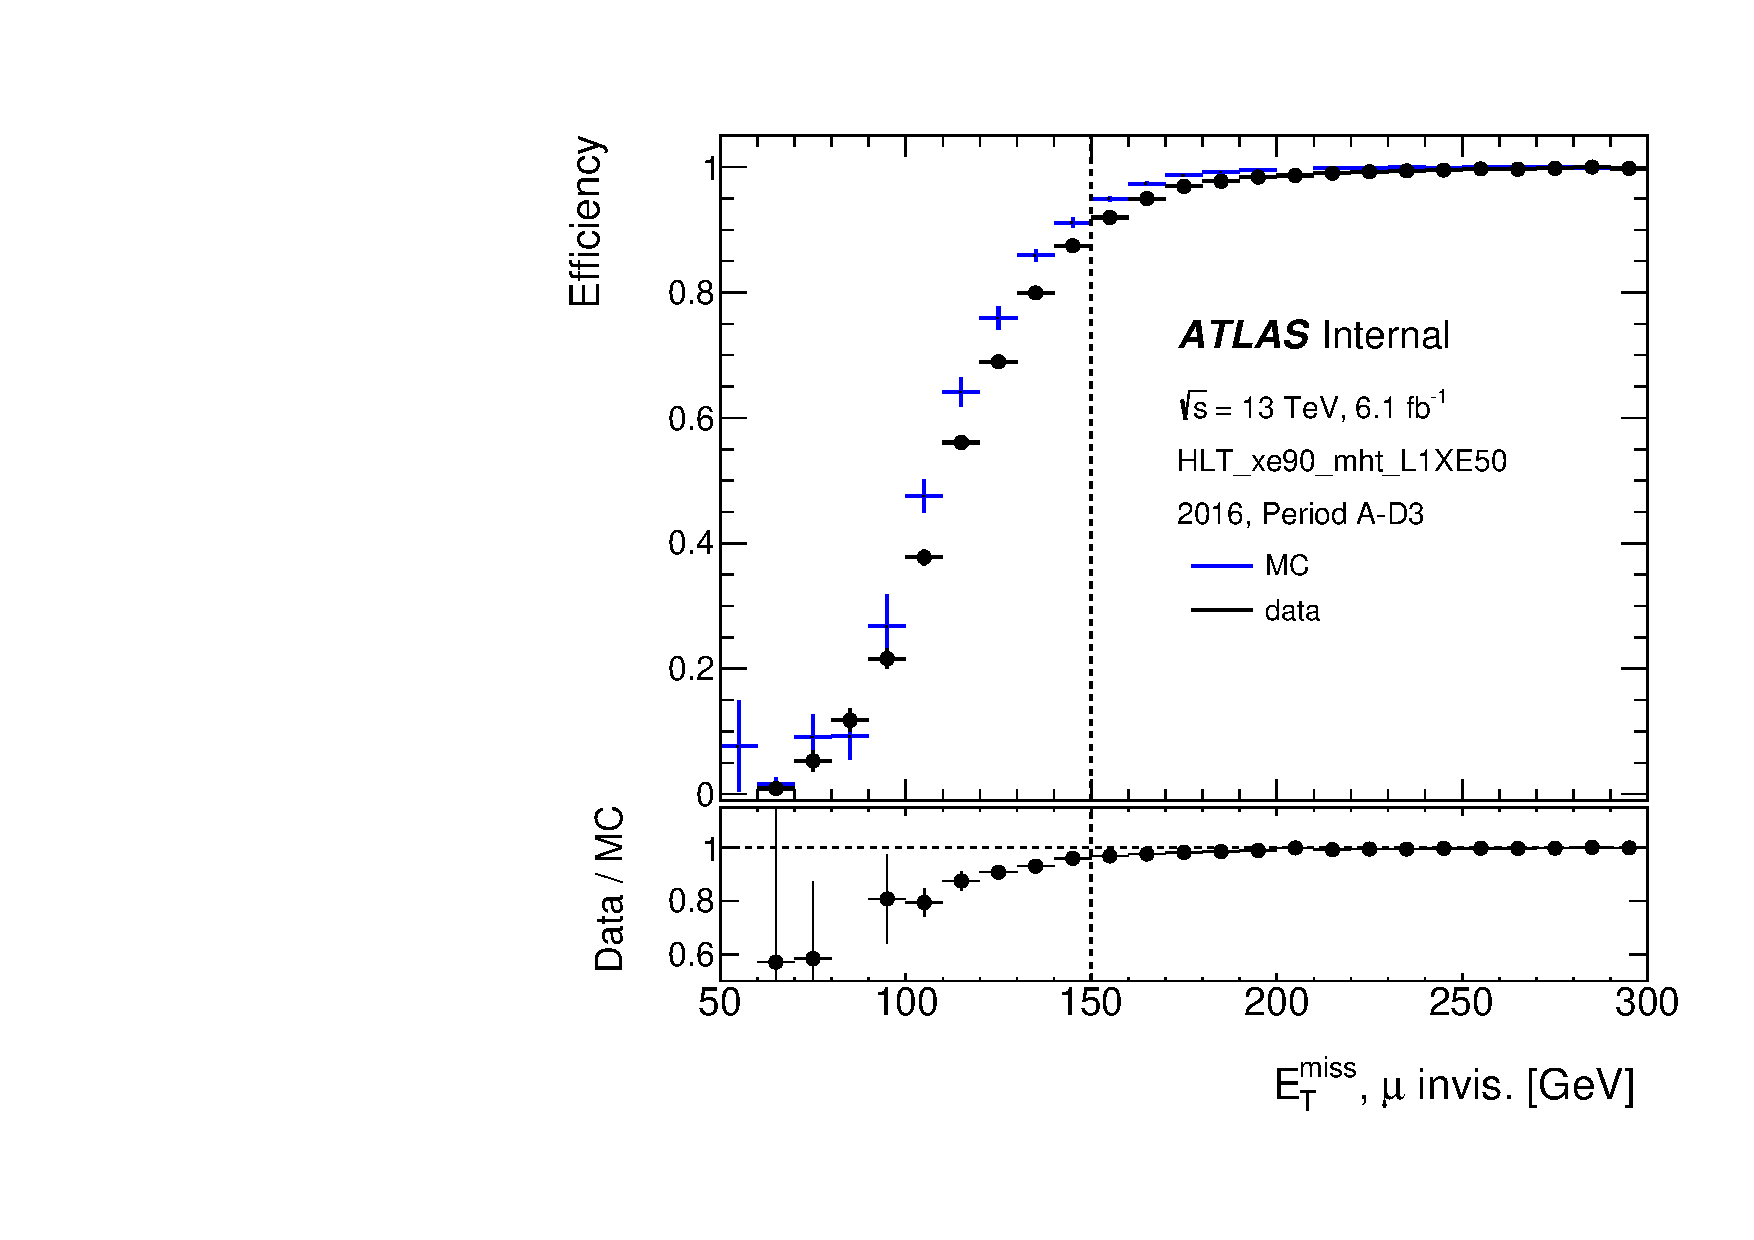
\includegraphics[width=0.45\textwidth]{chapters/c6/figures/METTriggerCalibration/efficiecy_HLT_xe90_mht_L1XE50.pdf}
	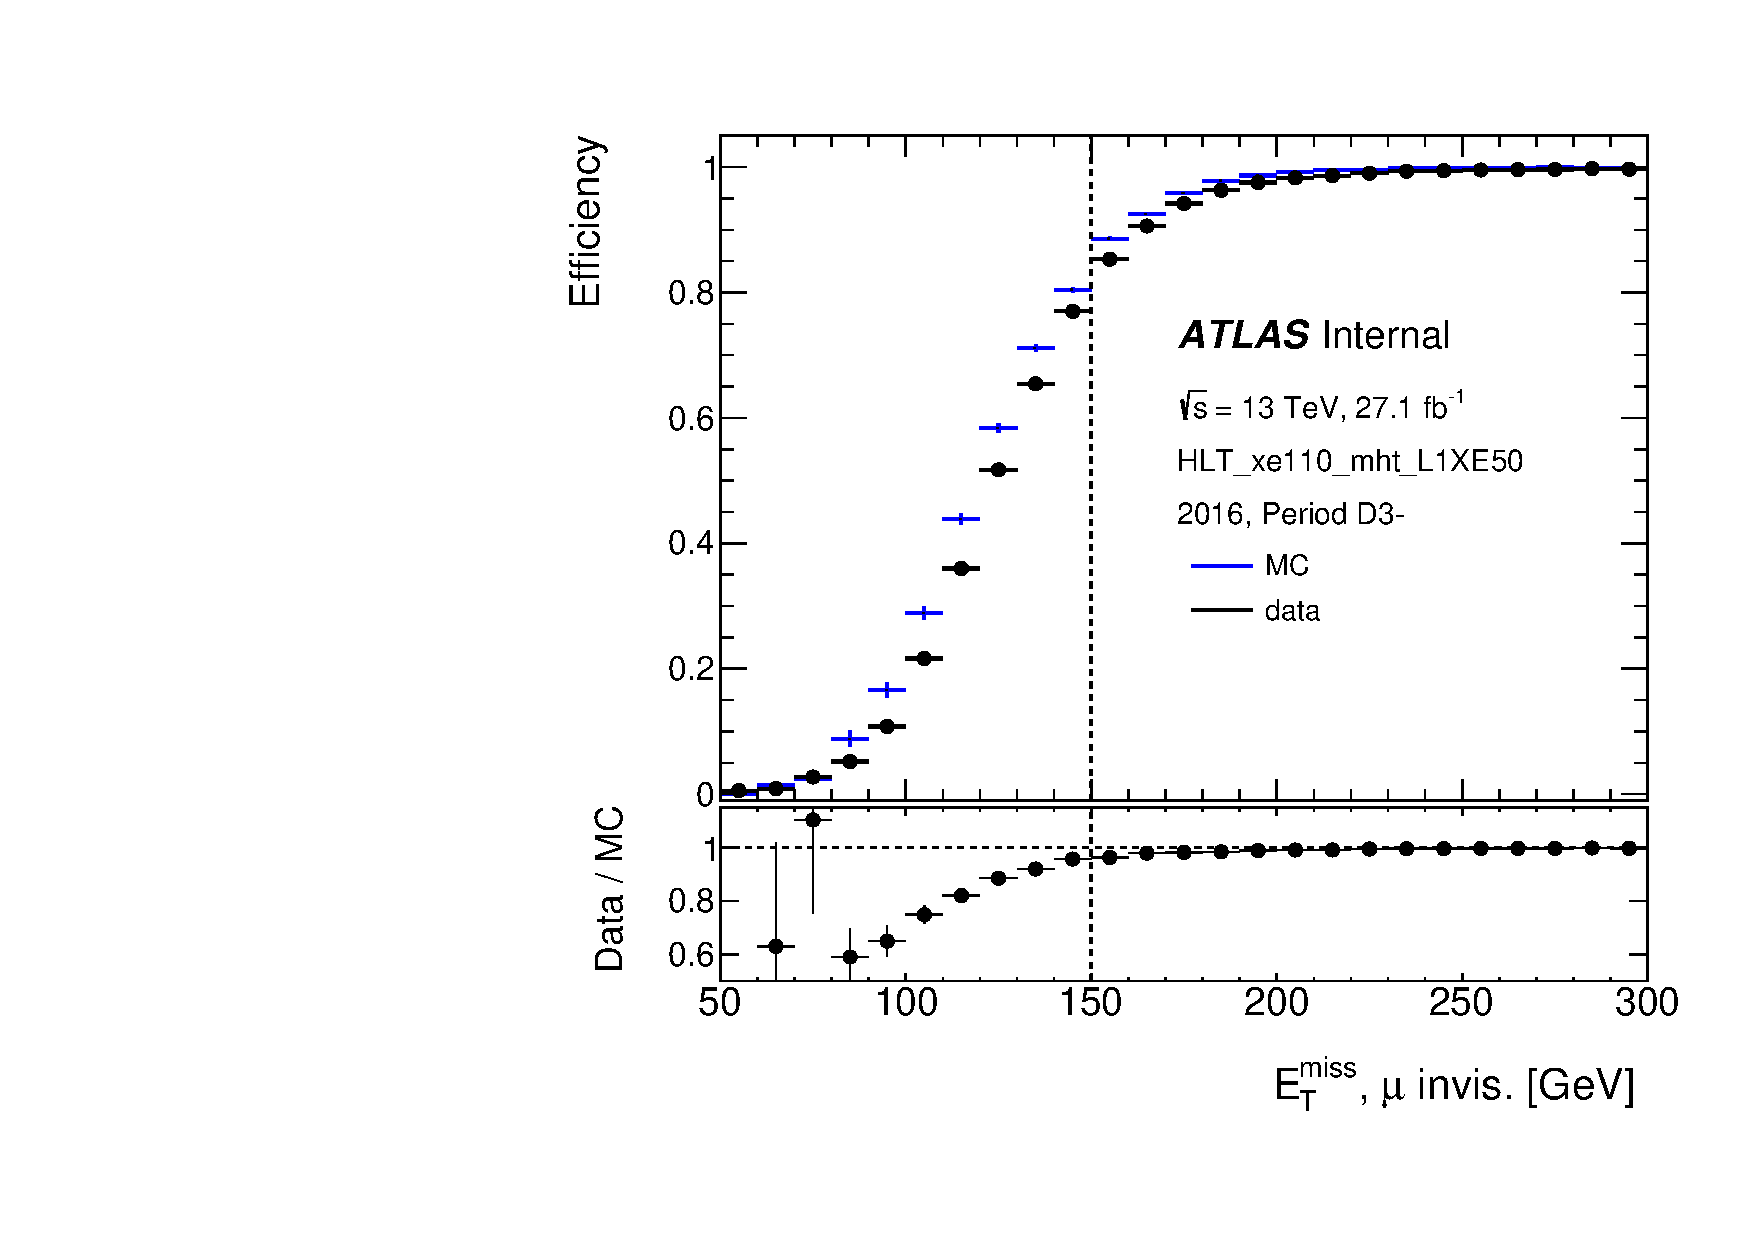
\includegraphics[width=0.45\textwidth]{chapters/c6/figures/METTriggerCalibration/efficiecy_HLT_xe110_mht_L1XE50.pdf}
	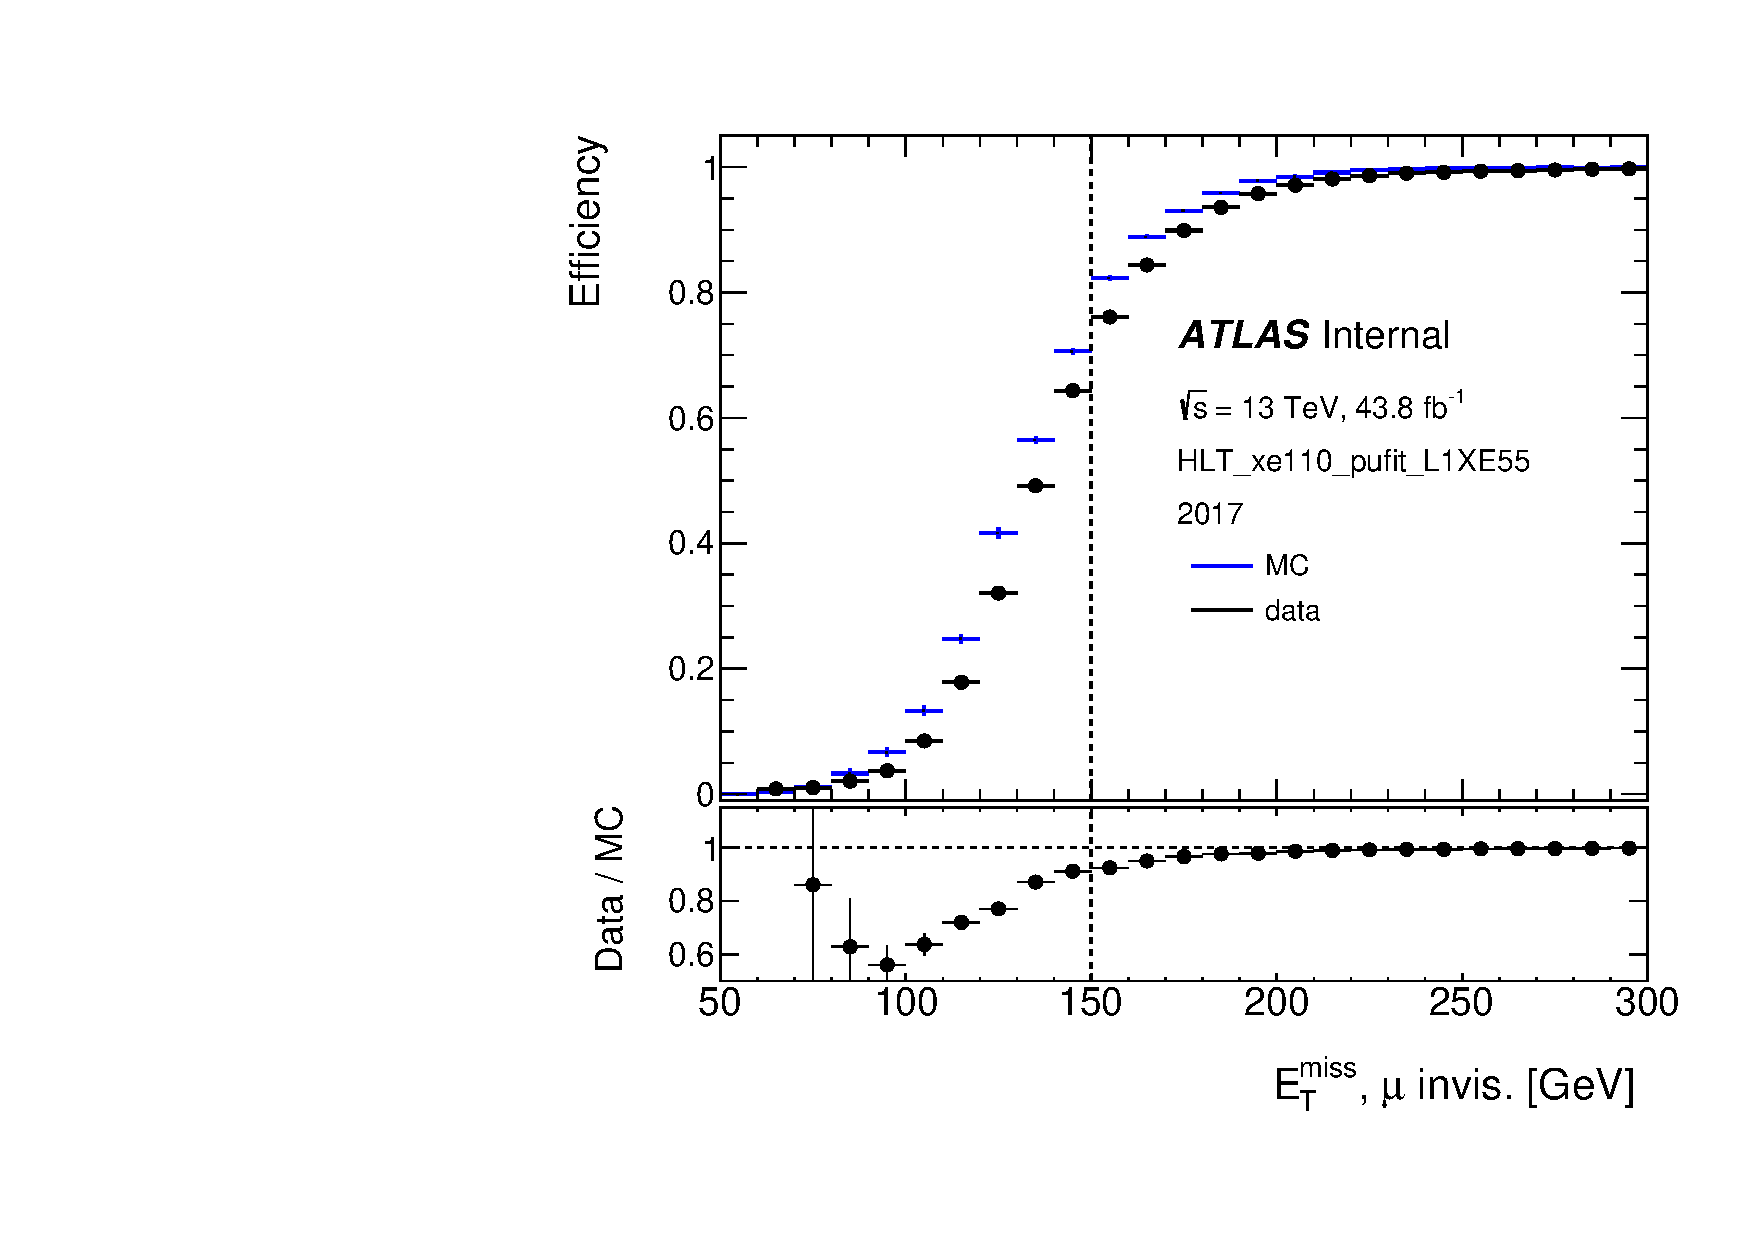
\includegraphics[width=0.45\textwidth]{chapters/c6/figures/METTriggerCalibration/efficiecy_HLT_xe110_pufit_L1XE55.pdf}
	\caption{Measured trigger efficiencies as a function of offline \METnomu~in data and MC for the \MET~triggers used in 2015-2018. The plots are shown for 0,1 and 2 tags together. The lower panels provide the ratio of data and MC events (the scale factor).}
	\label{fig:TrigEff}
\end{figure}

\par Scale factors (SF) are defined as the ratio of \MET~trigger efficiencies for data and MC:

\begin{equation}
	\label{eq:dataMCsf}
	\text{SF} = \frac{\text{Efficiency}^{\text{data}}_{\mu}}{\text{Efficiency}^{\text{MC}}_{\mu}}
\end{equation}

To calculate the data-driven corrections for the MC trigger turn-on curves, the scale factors are fitted for each \MET~trigger starting in the range $100~\GeV < \METnomu~< 300~\GeV$ in \MET~bins of 10~\GeV using the following fit function:

\begin{eqnarray}
	\label{eq:dataMCsf_fit}
	f\left(\text{x}\right) = p_0 \cdot \left[1 + \text{erf}\left(\frac{\text{x} - p_{1}}{\sqrt{2}p_{2}}\right)\right] + p_3
\end{eqnarray}
where $x = \METnomu$.

\par The scale factor applied to the MC in the signal region and one-lepton control region is given by evaluating $f(\met)$ or $f(\METnomu)$, respectively. 
The scale factors measured for the different \MET~are shown in Fig.~\ref{fig:TrigSF} together with the fitted SF curves.
Good agreement is observed in data and MC efficiencies comparison in Figure~\ref{fig:TrigSF_validation}, after the scale factors are applied to the simulation.

\begin{figure}[tb!]
	\centering
	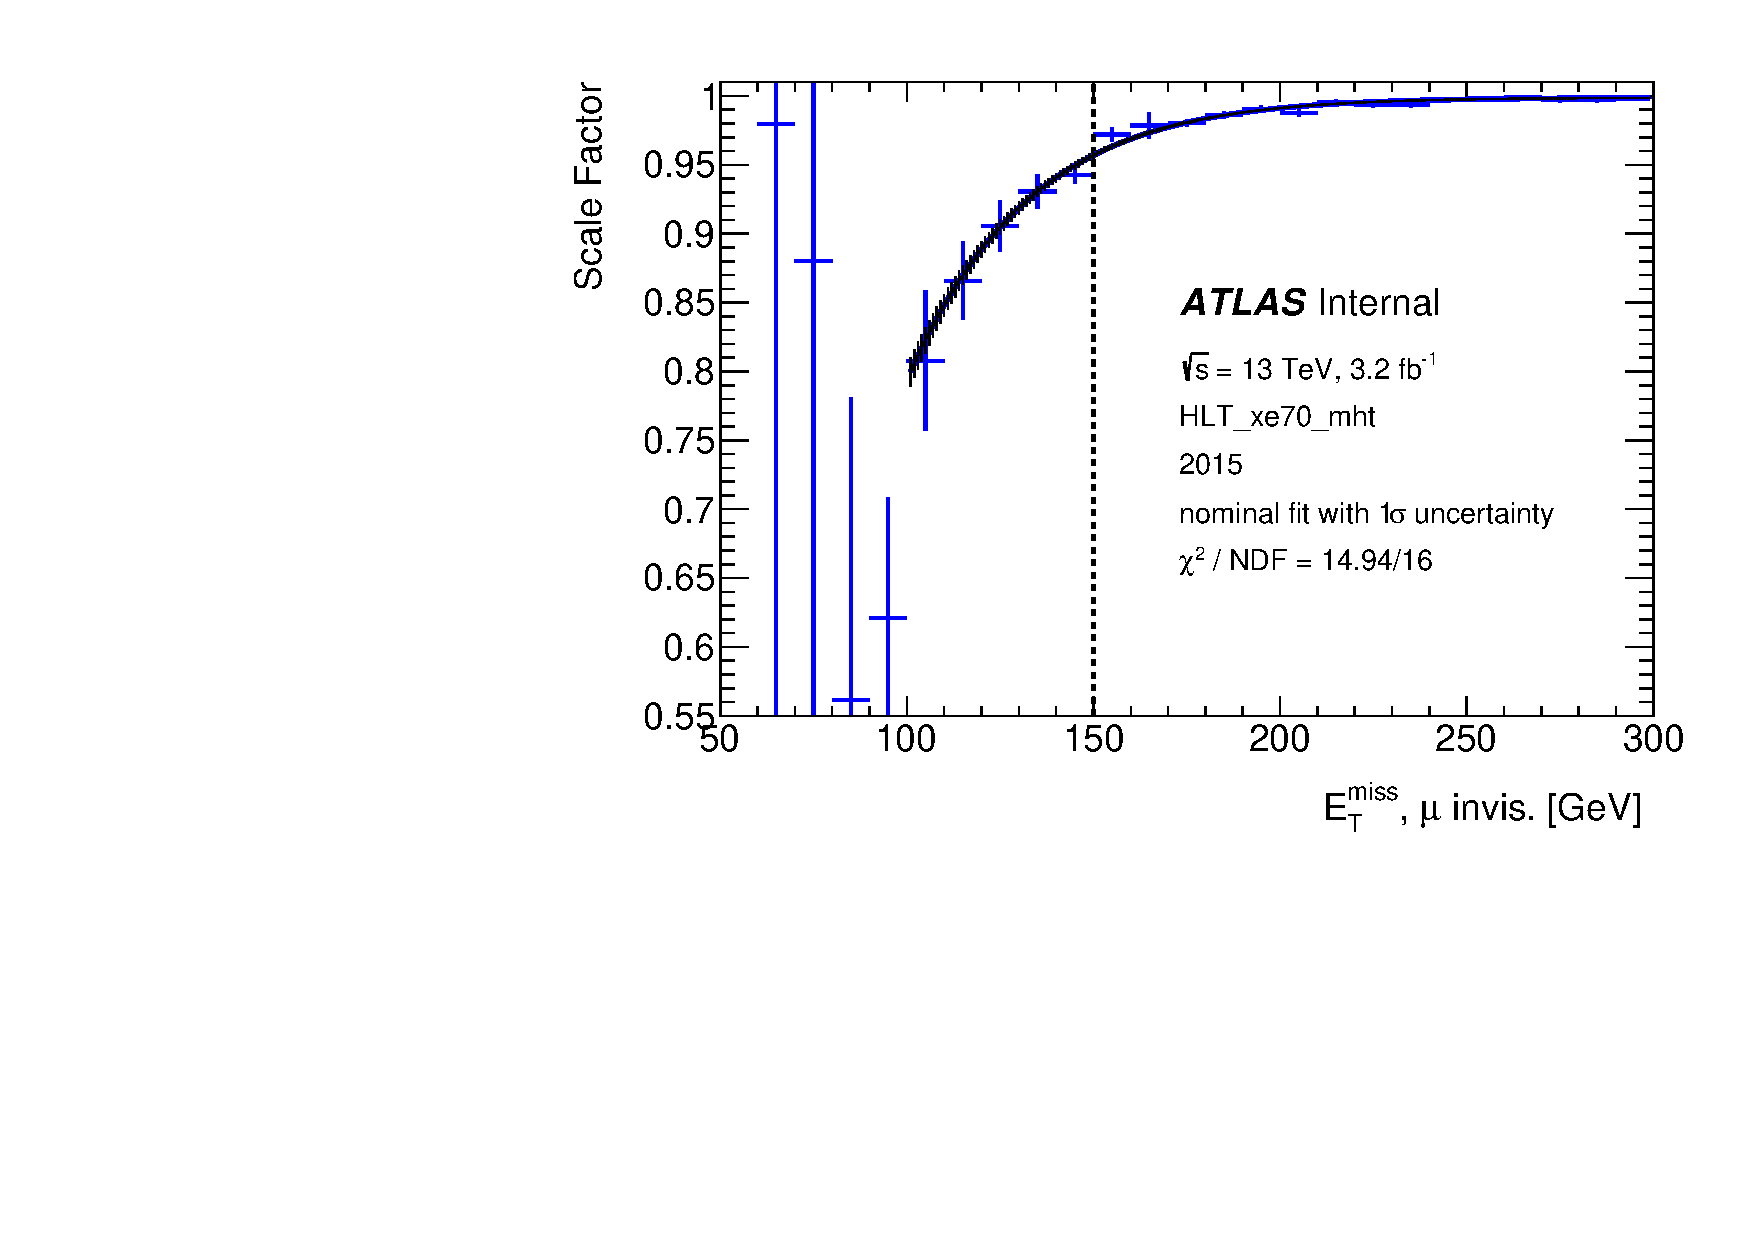
\includegraphics[width=0.45\textwidth]{chapters/c6/figures/METTriggerCalibration/SF_HLT_xe70_mht.pdf}
	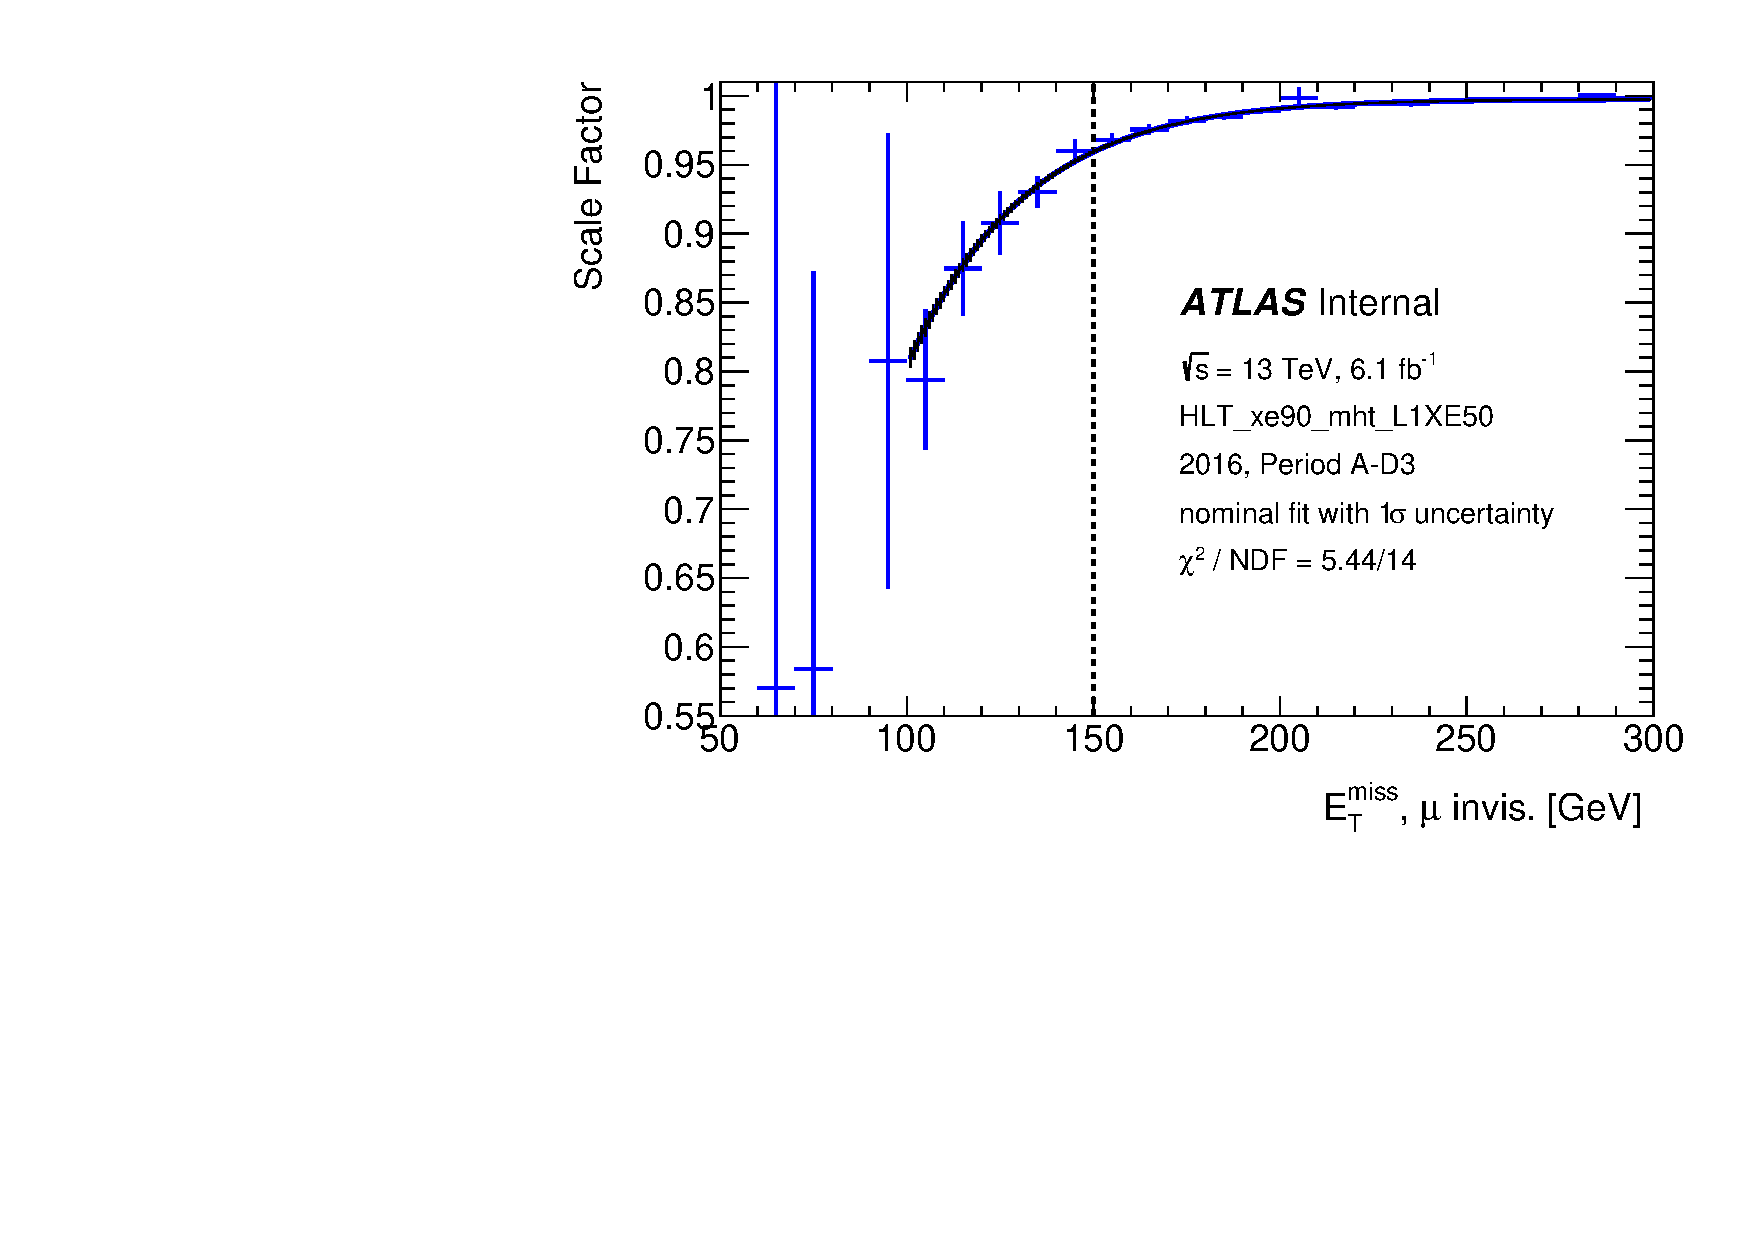
\includegraphics[width=0.45\textwidth]{chapters/c6/figures/METTriggerCalibration/SF_HLT_xe90_mht_L1XE50.pdf}
	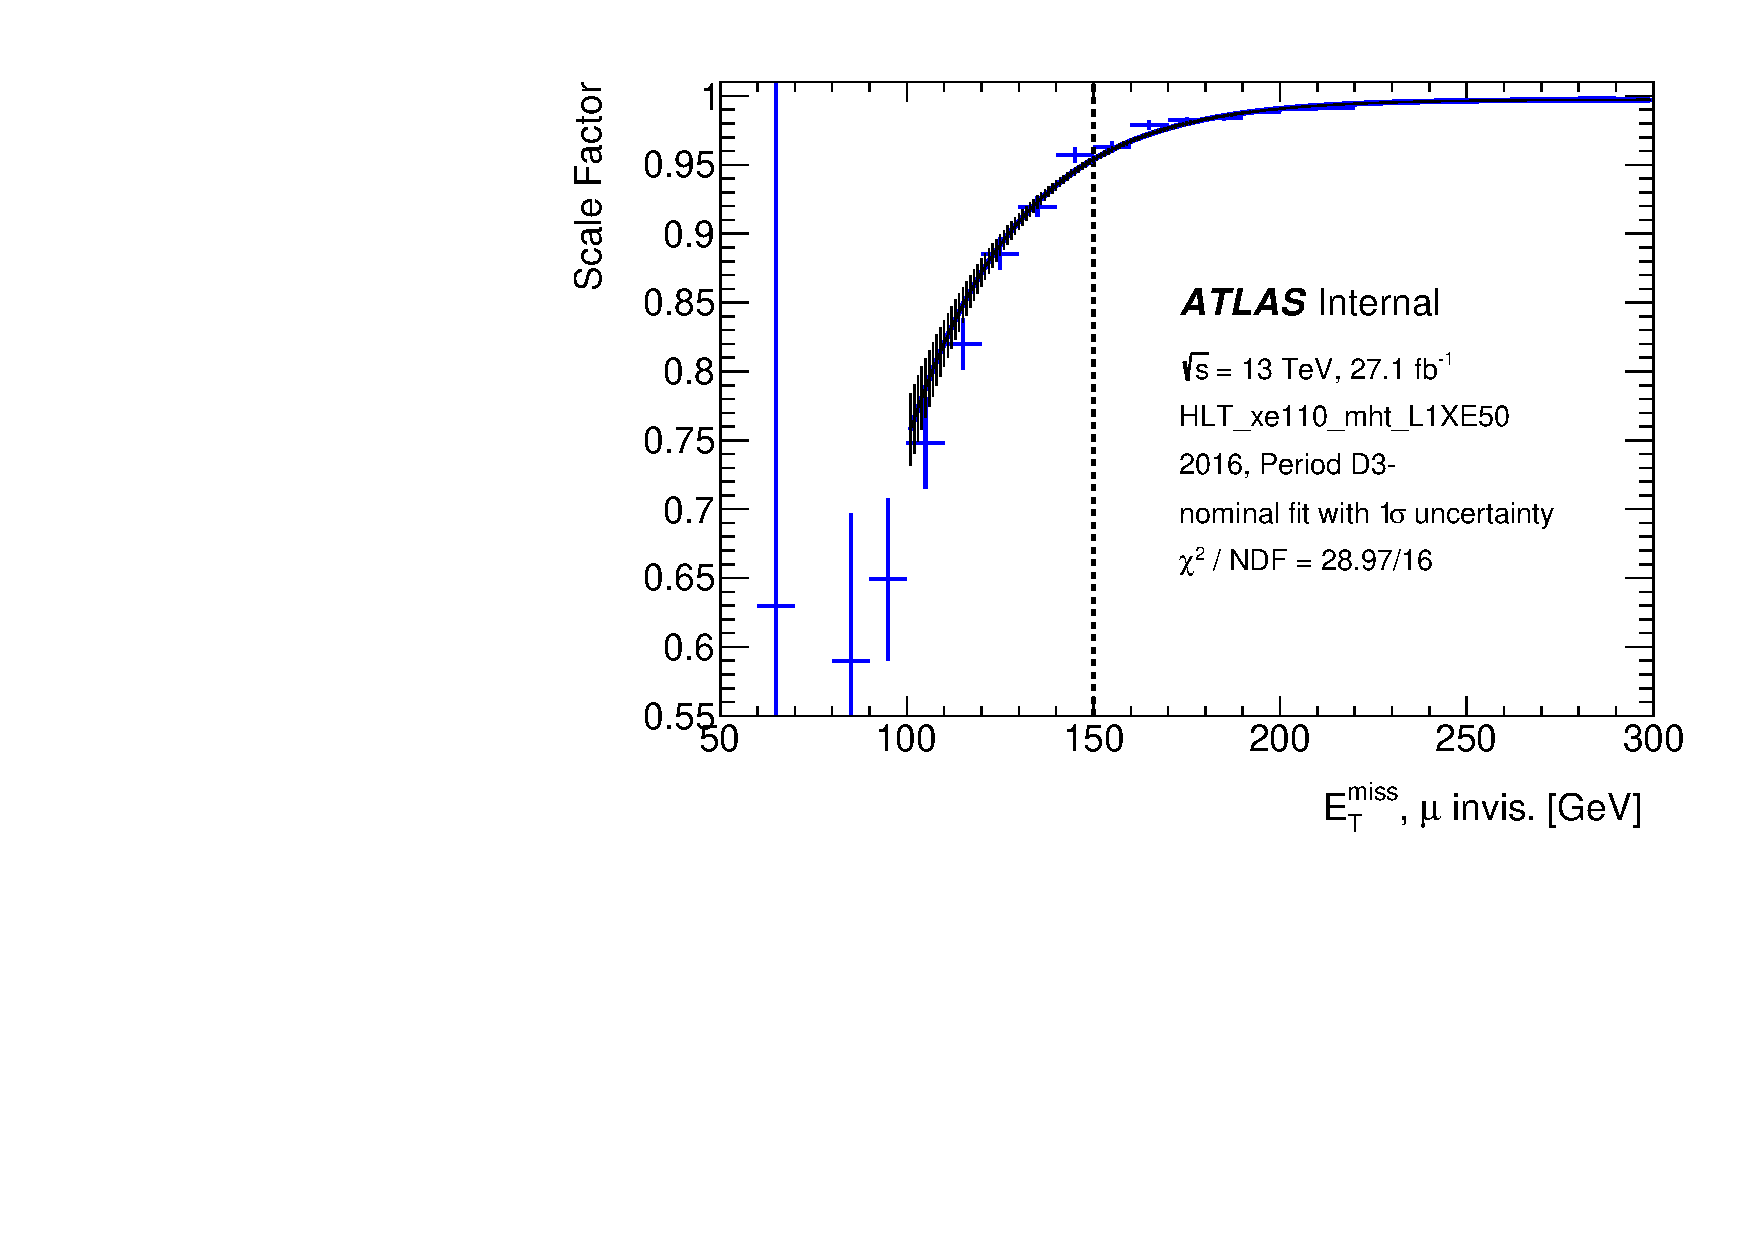
\includegraphics[width=0.45\textwidth]{chapters/c6/figures/METTriggerCalibration/SF_HLT_xe110_mht_L1XE50.pdf}
	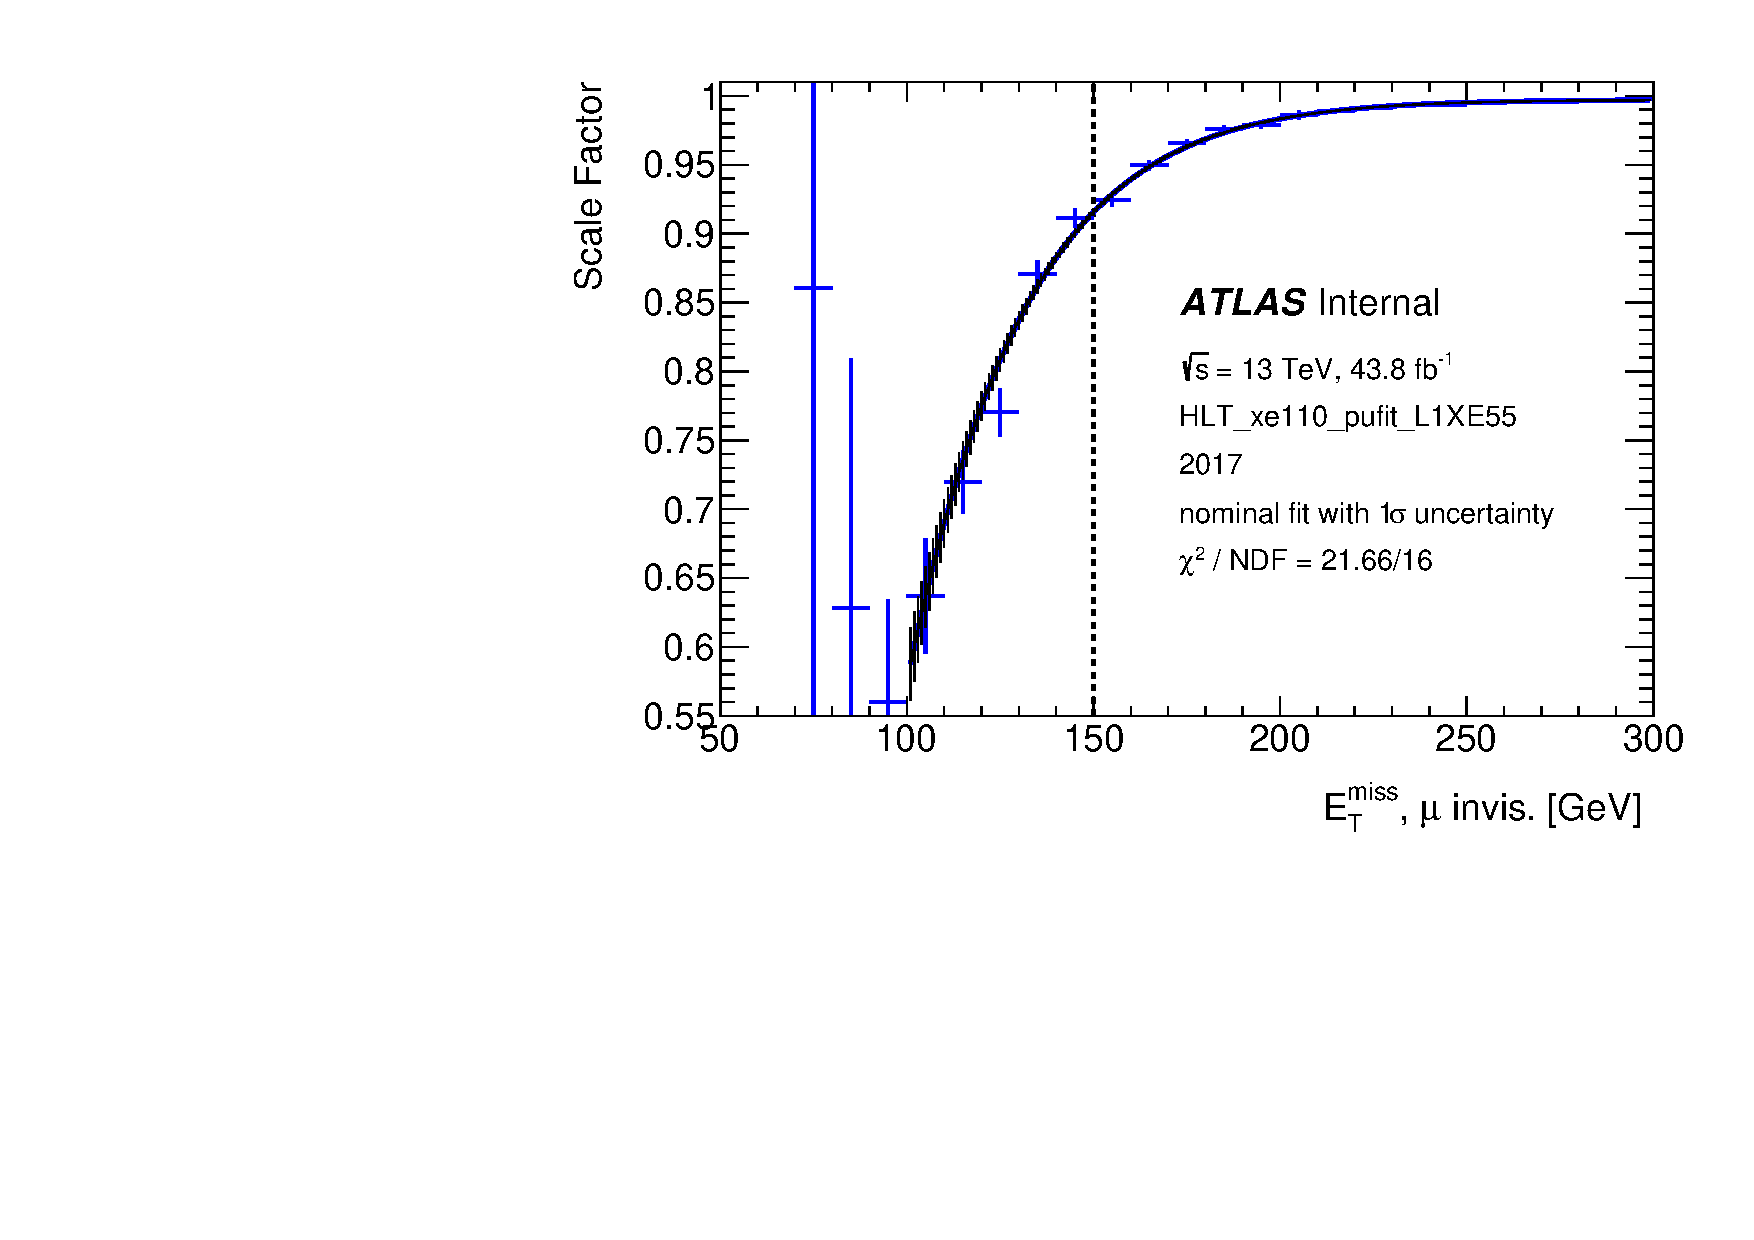
\includegraphics[width=0.45\textwidth]{chapters/c6/figures/METTriggerCalibration/SF_HLT_xe110_pufit_L1XE55.pdf}
	\caption{Measured scale factors as a function of offline \METnomu~for the \MET~triggers used in 2015-2010. The scale factors were derived for 0,1 and 2 tags together. The hatched band shows the 1$\sigma$ fit uncertainty.}
	\label{fig:TrigSF}
\end{figure}

\begin{figure}[tb!]
	\centering
	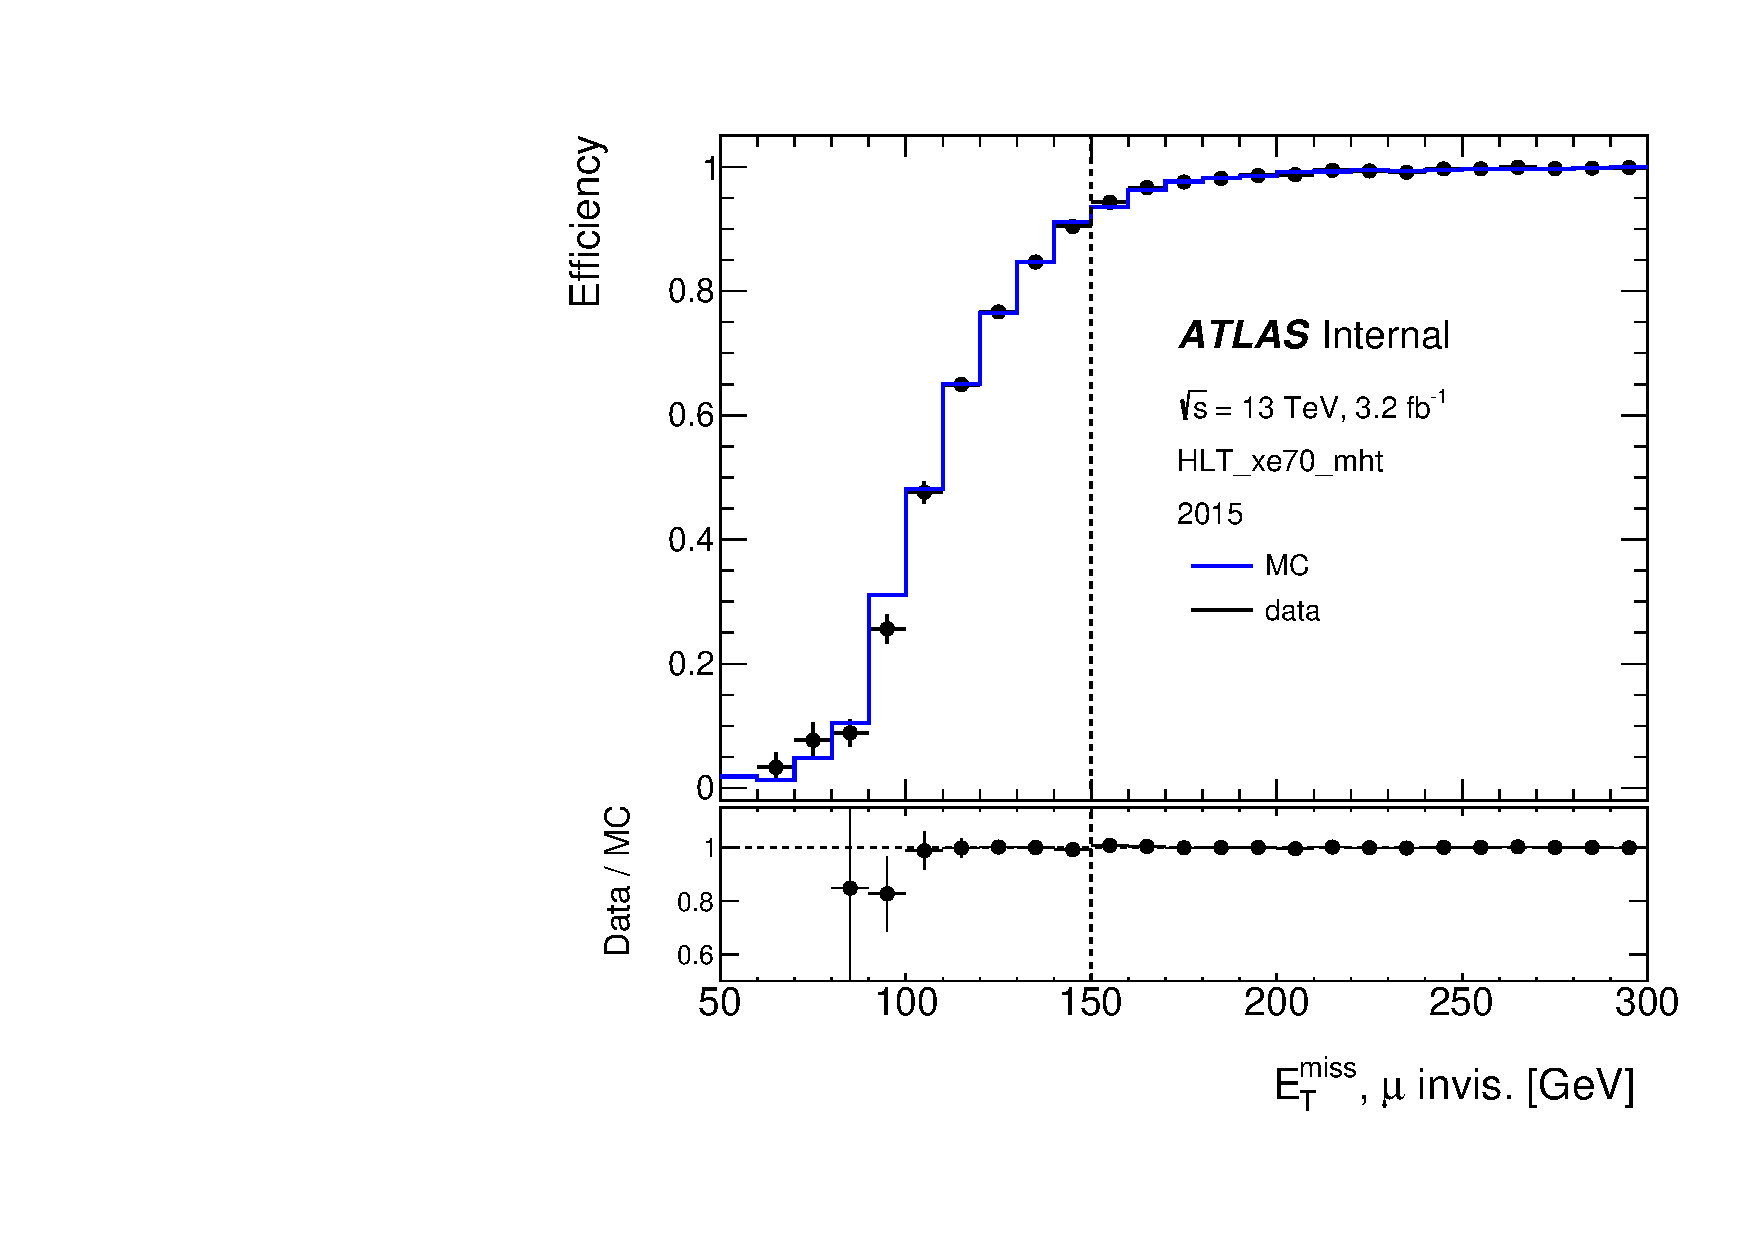
\includegraphics[width=0.45\textwidth]{chapters/c6/figures/METTriggerCalibration/validation_HLT_xe70_mht.pdf}
	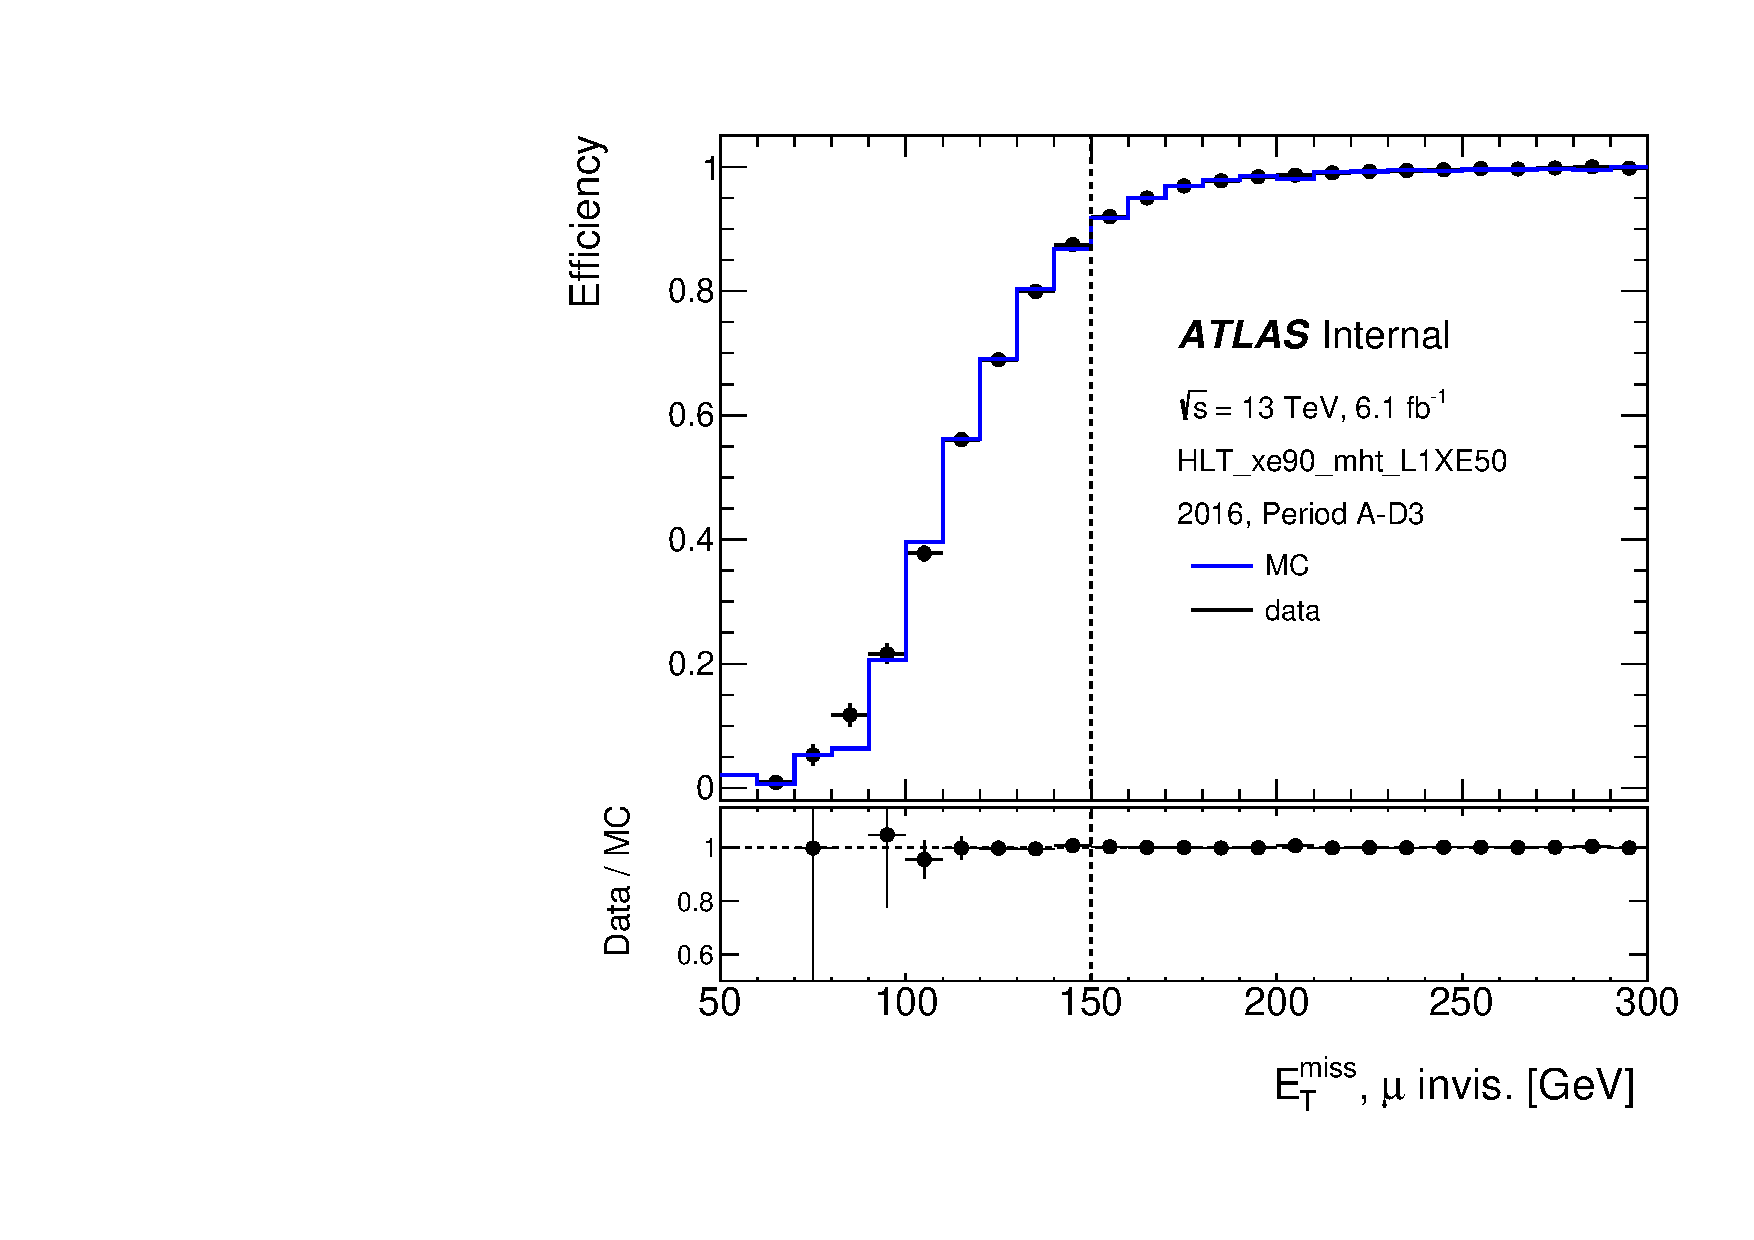
\includegraphics[width=0.45\textwidth]{chapters/c6/figures/METTriggerCalibration/validation_HLT_xe90_mht_L1XE50.pdf}
	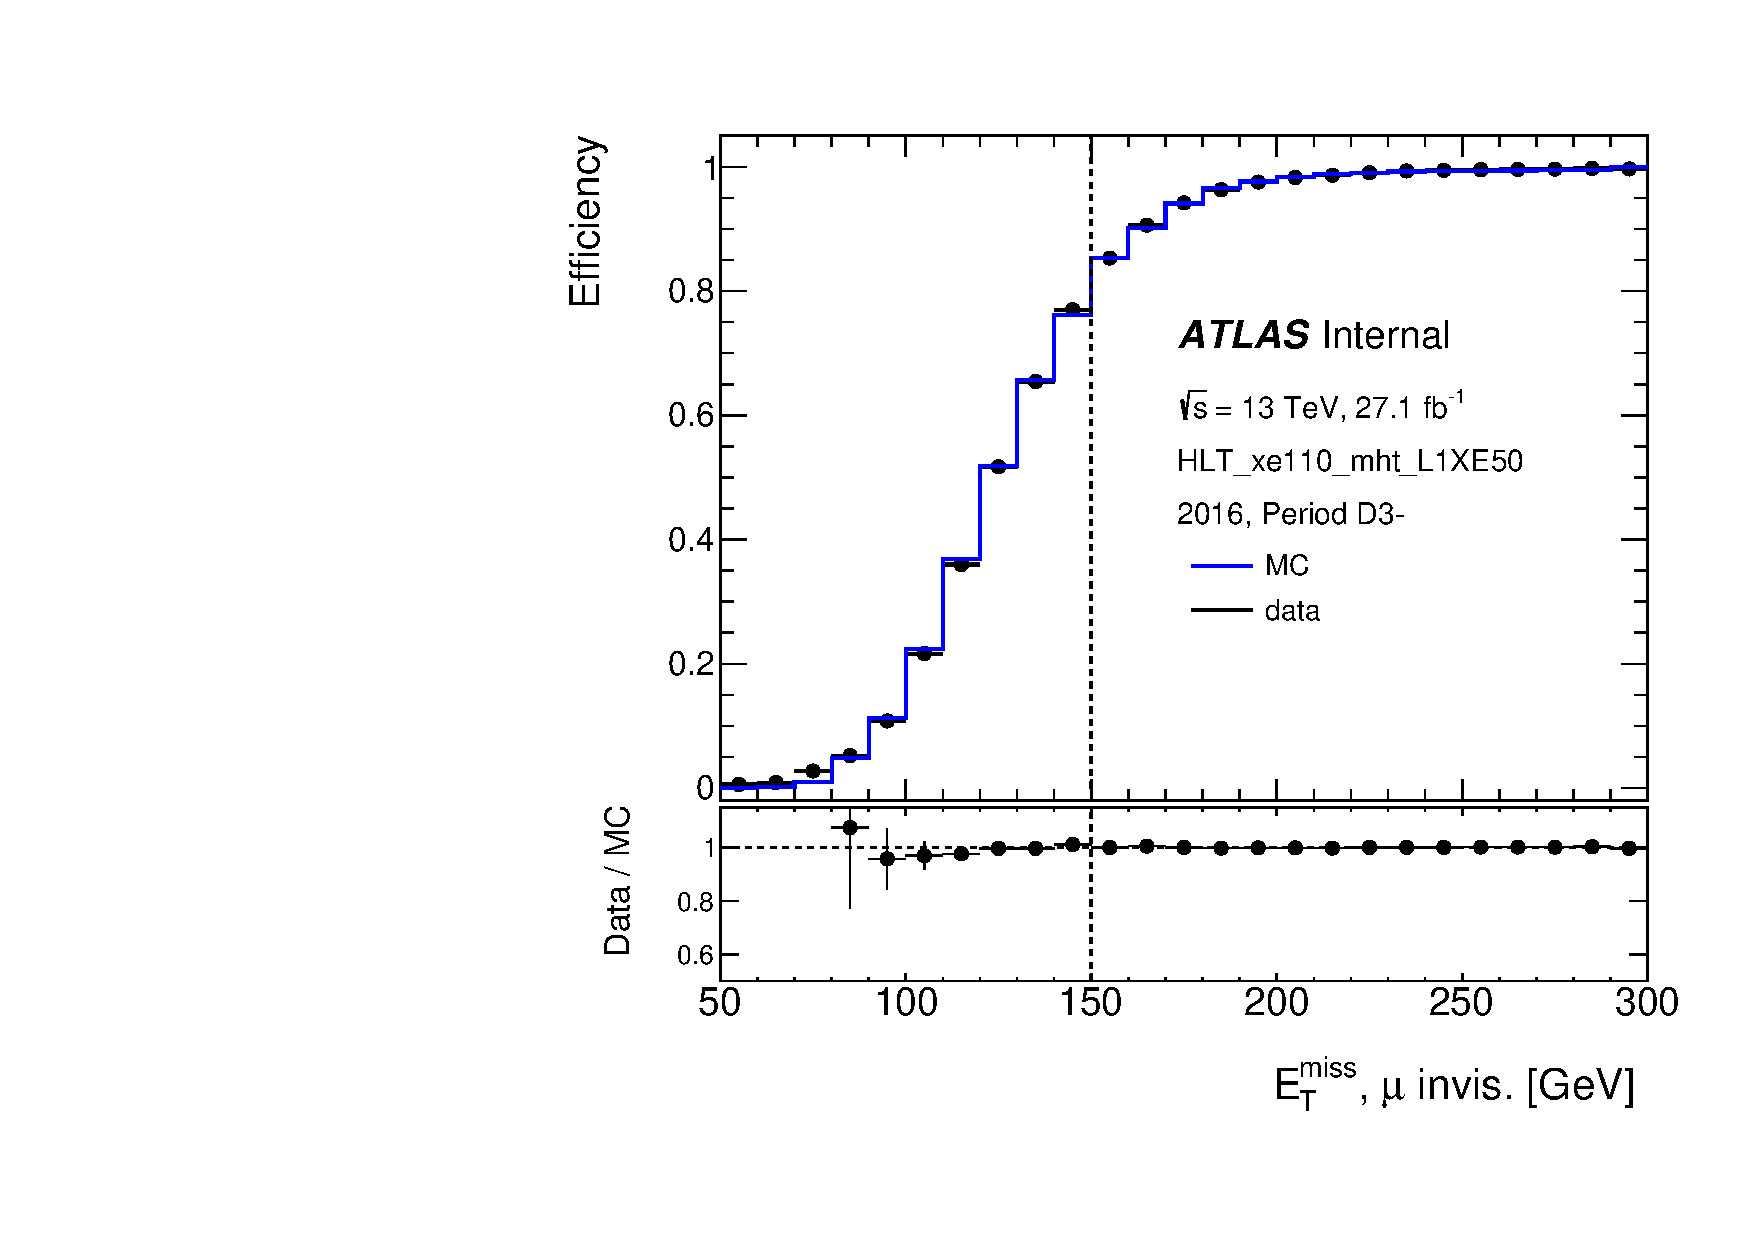
\includegraphics[width=0.45\textwidth]{chapters/c6/figures/METTriggerCalibration/validation_HLT_xe110_mht_L1XE50.pdf}
	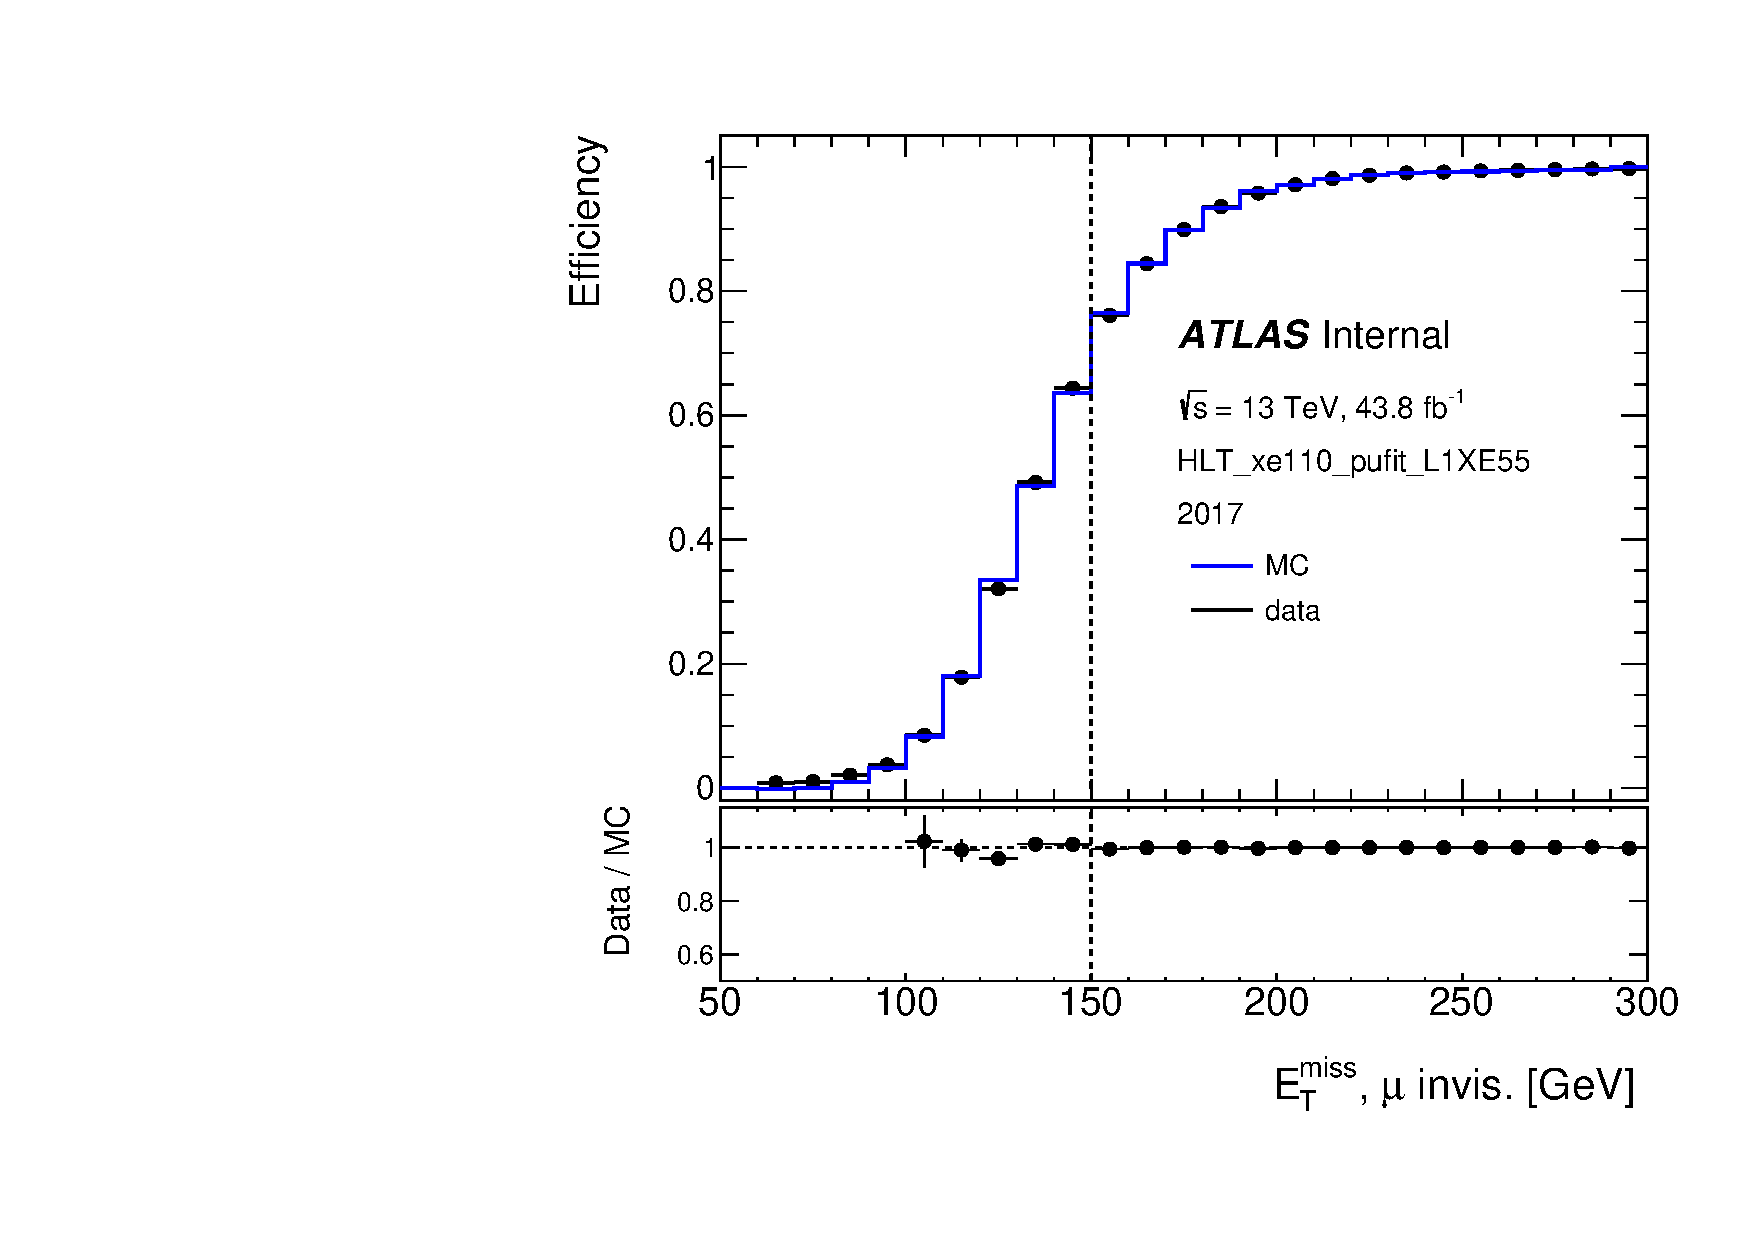
\includegraphics[width=0.45\textwidth]{chapters/c6/figures/METTriggerCalibration/validation_HLT_xe110_pufit_L1XE55.pdf}
	\caption{Validation plots showing \MET~trigger efficiencies and scale factors as function of offline \METnomu~after applying scale factor corrections for $\METnomu>100\,\GeV$ to the MC in the full single lepton region. Good agreement is observed between data and MC.}
	\label{fig:TrigSF_validation}
\end{figure}

\par The triggers are listed in Table~\ref{tab:summary_triggers_used}. 

\begin{table}
	\scriptsize
	\begin{center}
	    \resizebox{1.\textwidth}{!}{
			\begin{tabular}{c c c c}
				\hline
			    \hline
			    Period & 0 lepton & 1 lepton & 2 lepton + \met~trigger SF measurement \\
			    \hline
			    2015 & \textsc{HLT\_xe70\_mht} & \textsc{HLT\_xe70\_mht} & \textsc{HLT\_e24\_lhmedium\_L1EM20VH}\\
			    & & & \textbf{OR} \textsc{HLT\_e120\_lhloose}  \\ 
			    & & & \textbf{OR} \textsc{HLT\_mu20\_iloose\_L1MU15} \\
			    & & & \textbf{OR} \textsc{HLT\_mu50} \\
			    \hline
			    2016 & \textsc{HLT\_xe90\_mht\_L1XE50} & \textsc{HLT\_xe90\_mht\_L1XE50} & \textsc{HLT\_e60\_lhmedium\_nod0}  \\
			    (A) & & & \textbf{OR} \textsc{HLT\_e140\_lhloose\_nod0} \\ 
			    & & & \textbf{OR} \textsc{HLT\_mu40} \\
			    & & & \textbf{OR} \textsc{HLT\_mu50} \\
			    \hline
			    2016 & \textsc{HLT\_xe90\_mht\_L1XE50} & \textsc{HLT\_xe90\_mht\_L1XE50} & \\
                (B-D3) & & & \textsc{HLT\_e60\_lhmedium\_nod0} \\
			    & & & \textbf{OR} \textsc{HLT\_e140\_lhloose\_nod0} \\ 
			    & & & \textbf{OR} \textsc{HLT\_mu24\_ivarmedium} \\
			    & & & \textbf{OR} \textsc{HLT\_mu50} \\
			    \hline
			    2016 & \textsc{HLT\_xe110\_mht\_L1XE50} & \textsc{HLT\_xe110\_mht\_L1XE50} & \textsc{HLT\_e26\_lhtight\_nod0\_ivarloose} \\	
			    (D4-E3)& & & \textbf{OR} \textsc{HLT\_e60\_lhmedium\_nod0} \\
			    & & & \textbf{OR} \textsc{HLT\_e140\_lhloose\_nod0} \\ 
			    & & & \textbf{OR} \textsc{HLT\_mu24\_ivarmedium} \\
			    & & & \textbf{OR} \textsc{HLT\_mu26\_ivarmedium} \\
			    & & & \textbf{OR} \textsc{HLT\_mu50} \\
		        \hline
			    2016 & \textsc{HLT\_xe110\_mht\_L1XE50} & \textsc{HLT\_xe110\_mht\_L1XE50} & \textsc{HLT\_e26\_lhtight\_nod0\_ivarloose}\\
                (F1)&  & & \textbf{OR} \textsc{HLT\_e60\_lhmedium\_nod0} \\
			    & & & \textbf{OR} \textsc{HLT\_e140\_lhloose\_nod0} \\ 
			    & & & \textbf{OR} \textsc{HLT\_mu26\_ivarmedium} \\
			    & & & \textbf{OR} \textsc{HLT\_mu50} \\
			    \hline
			    2016 & \textsc{HLT\_xe110\_mht\_L1XE50} & \textsc{HLT\_xe110\_mht\_L1XE50} &\textsc{HLT\_e26\_lhtight\_nod0\_ivarloose} \\
			    (F2-) & & & \textbf{OR} \textsc{HLT\_e60\_lhmedium\_nod0} \\
			    & & & \textbf{OR} \textsc{HLT\_e140\_lhloose\_nod0} \\ 
			    & & & \textbf{OR} \textsc{HLT\_mu26\_ivarmedium} \\
			    & & & \textbf{OR} \textsc{HLT\_mu50} \\
			    \hline
			    2017 & \textsc{HLT\_xe110\_pufit\_L1XE55} & \textsc{HLT\_xe110\_pufit\_L1XE55} &\textsc{HLT\_e60\_lhmedium\_nod0} \\
			    & & & \textbf{OR} \textsc{HLT\_e140\_lhloose\_nod0} \\
			    & & & \textbf{OR} \textsc{HLT\_mu26\_ivarmedium} \\
			    & & & \textbf{OR} \textsc{HLT\_mu50} \\
			    \hline
			    2018 & \textsc{HLT\_xe110\_pufit\_70\_L1XE55} & \textsc{HLT\_xe110\_pufit\_70\_L1XE55} &  \textsc{HLT\_e60\_lhmedium\_nod0} \\
			    (B-C5)& & & \textbf{OR} \textsc{HLT\_e140\_lhloose\_nod0} \\
			    & & & \textbf{OR} \textsc{HLT\_mu26\_ivarmedium} \\
			    & & & \textbf{OR} \textsc{HLT\_mu50} \\
			    \hline
			    2018 & \textsc{HLT\_xe110\_pufit\_65\_L1XE55} & \textsc{HLT\_xe110\_pufit\_65\_L1XE55} &\textsc{HLT\_e60\_lhmedium\_nod0} \\
			    (C5-) & & & \textbf{OR} \textsc{HLT\_e140\_lhloose\_nod0} \\
			    & & & \textbf{OR} \textsc{HLT\_mu26\_ivarmedium} \\
			    & & & \textbf{OR} \textsc{HLT\_mu50} \\    		
			    \hline
			    \hline
		    \end{tabular}
		}
	\end{center}
	\caption{\met~and single-lepton triggers used in the analysis.}
	\label{tab:summary_triggers_used}
\end{table}
	
\section{MC samples}
\label{ch:data-mc-samples}

\subsection{2HDM+a and Z'-2HDM signal}
\label{subsec:signal}

\par Simulated events corresponding to the $pp\to h\chi\bar{\chi}$ process were generated with \textsc{MadGraph5\_aMC@NLO} (\textsc{MG5\_aMC}) 2.6.1 \cite{Alwall:2014hca} 
based on the UFO model developed in \cite{Abe:2018bpo} at leading-order (LO) accuracy using the NNPDF 3.0 next-to-leading order~(NLO) PDF set with $\alpha_s=0.118$ \cite{Ball:2014uwa}. 
The signal samples are generated separately for the loop-induced gluon--gluon fusion (ggF) process and the $b$-initiated production. 

\par Simulated events corresponding to the $pp\to Z'\to h A(\chi\bar{\chi})$ process were generated with \textsc{MadGraph5\_aMC@NLO} (\textsc{MG5\_aMC}) 2.2.3 \cite{Alwall:2014hca} 
at leading-order (LO) accuracy using the NNPDF 2.3 NLO PDF set with $\alpha_s=0.119$ \cite{Ball:2012cx}. 
The 4-flavour scheme was used for the calculation of the matrix elements. Several samples were generated for different values of $m(Z')$ and $m(A)$.
The masses of the additional Higgs bosons were fixed to $m(H)=m(H^{\pm})=300$ GeV and the mass of the DM candidates was fixed to $m(\chi)=100$ GeV. 

\par The parton shower and hadronisation were simulated with \textsc{Pythia} 8.230 \cite{Sjostrand:2014zea} and \textsc{Pythia} 8.186 \cite{Sjostrand:2007gs}, respectively for 2HDM+a and Z' 2HDM signal,
using the A14 set \cite{ATL-PHYS-PUB-2014-021} of tuned parameters together with the NNPDF 2.3 LO PDF set \cite{Ball:2011mu}. 
Higgs boson decays into $b\bar{b}$ pairs were also simulated with according \textsc{Pythia} versions with a branching fraction fixed to the SM prediction.

\subsection{V+jets}

\par $V+$ jets production is simulated with the
\textsc{Sherpa} v2.2~\cite{Bothmann:2019yzt} generator. In this setup, NLO-accurate
matrix elements for up to two jets, and LO-accurate matrix elements for up
to four jets are calculated with the Comix~\cite{Gleisberg:2008fv} and
OpenLoops~\cite{Cascioli:2011va,Denner:2016kdg} libraries. They are matched
with the \textsc{Sherpa} parton shower~\cite{Schumann:2007mg} using the MEPS@NLO
prescription~\cite{Hoeche:2011fd,Hoeche:2012yf,Catani:2001cc,Hoeche:2009rj}.
Samples are generated using the
\nnpdfnnlo set~\cite{Ball:2014uwa}.

\par The samples are split according to whether they contain a $B$ hadron or no $B$ with $p_T > 5$ GeV and $|\eta|<2.9$, a $C$ hadron with $p_T > 4$ GeV and $|\eta|<3$ 
(with the filtered samples called Bfilter, CFilterBVeto, CVetoBVeto respectively). They are further split by either:

\begin{itemize}
	\item using the transverse momentum of the $V$ boson produced by Sherpa ($p_T(V)$), or
	\item using the $\max{p_T(V),H_T}$, where $H_T$ is the scalar sum of the \pt~of the vector boson and the jets.
\end{itemize}%

\subsection{$t\bar{t}$}

\par The production of \ttbar\ events is modelled using the \powhegbox~\cite{Frixione:2007nw,Nason:2004rx,Frixione:2007vw,Alioli:2010xd}~v2
generator which provides matrix elements at NLO with the NNPDF3.0NLO~\cite{Ball:2014uwa} parton distribution function (PDF) and the \hdamp\ parameter\footnote{The \hdamp\ parameter
controls the transverse momentum \pt\ of the first additional emission beyond the leading-order Feynman diagram
in the parton shower and therefore regulates the  high-\pt\ emission against which the \ttbar\ system recoils.} set to 1.5~\mtop~\cite{ATL-PHYS-PUB-2016-020}.
The functional form of the renormalisation and factorisation scale is set to the default scale $\sqrt{m_{\textrm{top}}^2 + p_{\textrm T}^2}$.
The events are interfaced with \pythia.230~\cite{Sjostrand:2014zea} for the parton shower and hadronisation,
using the A14 set of tuned parameters~\cite{ATL-PHYS-PUB-2014-021}  and the NNPDF23LO PDF set.
The decays of bottom and charm hadrons are simulated using the \evtgen\ v1.6.0 program~\cite{EvtGen}.

\par The events are filtered to select dilepton or semi-leptonic $t\bar{t}$ decays. Two sets of samples are used in the analysis

\begin{itemize}
	\item an inclusive $t\bar{t}$ sample
	\item a set of \met-filtered $t\bar{t}$ samples, which was not used in the previous iteration of the analysis \cite{ATLAS-CONF-2018-039}, and was specifically developed to reduce the MC statistical uncertainties in the high-\met region.
\end{itemize}

\subsection{Single top}

\par Single-top $tW$ associated production, single-top t-channel and s-channel production are all modelled using the \powhegbox~\cite{Frederix:2012dh,Nason:2004rx,Frixione:2007vw,Alioli:2010xd}~v2
generator which provides matrix elements at NLO\
with the NNPDF3.0NLOnf4~\cite{Ball:2014uwa} PDF set.
The diagram removal scheme~\cite{Frixione:2008yi} was employed to handle the interference with \ttbar\ production~\cite{ATL-PHYS-PUB-2016-020}.
The events are interfaced with \pythia.230~\cite{Sjostrand:2014zea} using the A14 tune~\cite{ATL-PHYS-PUB-2014-021} and the NNPDF23LO PDF set.
The decays of bottom and charm hadrons are simulated using the \evtgen\ v1.6.0 program~\cite{EvtGen}.
For the t-channel, the functional form of the renormalisation and factorisation scale is set to $\sqrt{m_{\textrm{b}}^2 + p_{{\textrm T},b}^2}$
following the recommendation of~\cite{Frederix:2012dh} while for the other two, the functional form of the renormalisation and factorisation scale is set to the default scale, which is equal to the top-quark mass.

\subsection{Diboson}

\par Semileptonically decaying diboson and loop-induced diboson samples are simulated with the
\sherpa~v2.2~\cite{Bothmann:2019yzt} generator. In this setup multiple
matrix elements are matched and merged with the \sherpa parton shower
based on Catani-Seymour dipole~\cite{Gleisberg:2008fv,Schumann:2007mg}
using the MEPS@NLO
prescription~\cite{Hoeche:2011fd,Hoeche:2012yf,Catani:2001cc,Hoeche:2009rj}. 
The virtual QCD correction for matrix elements at NLO accuracy are
provided by the \openloops\ library~\cite{Cascioli:2011va,Denner:2016kdg}. 
library~\cite{Denner:2016kdg}. Samples are generated using the
\nnpdfnnlo set~\cite{Ball:2014uwa}.

\subsection{SM $Vh(b\bar{b})$}

\par The production of $q\bar{q}\to Wh\to \ell\nu b\bar{b}$ and $q\bar{q}\to Zh\to \ell\ell b\bar{b}$ events is modelled using the \powhegbox v2 generator
\cite{Alioli:2010xd} using the \minlo procedure \cite{Hamilton:2012np,Luisoni:2013kna} with the NNPDF3.0NLO~\cite{Ball:2014uwa} PDF set.
The events are interfaced with \pythia.212~\cite{Sjostrand:2014zea}~ using the AZNLO tune~\cite{Aad:2014xaa} and the CTEQ6L1~\cite{Pumplin:2002vw} PDF set.

\par The loop-induced $gg\to Zh \to \ell b\bar{b}, \nu\bar{\nu}b\bar{b}$ process is modelled using the \powhegbox v2 generator \cite{Alioli:2010xd} with the NNPDF3.0NLO~\cite{Ball:2014uwa} PDF set.
Parton showering and hadronisation are provided by \pythia.212~\cite{Sjostrand:2014zea} with the same settings as the one used for the $q\bar{q}$ process.

\subsection{$t\bar{t}+Z/H$}

\par \ttH\ events is modelled using the \powhegbox~\cite{Frixione:2007nw,Nason:2004rx,Frixione:2007vw,Alioli:2010xd,Hartanto:2015uka}
generator at NLO with the NNPDF3.0NLO~\cite{Ball:2014uwa} PDF set.
The events are interfaced with \pythia.230~\cite{Sjostrand:2014zea}~ using the A14 tune~\cite{ATL-PHYS-PUB-2014-021} and the NNPDF2.3LO~\cite{Ball:2014uwa} PDF set.

\par \ttV\ events is modelled using the \mgamc~v2.3.3 \cite{Alwall:2014hca}
generator which provides matrix elements at next-to-leading order~(NLO) 
with the NNPDF3.0NLO~\cite{Ball:2014uwa} parton distribution function~(PDF).
The functional form of the renormalization and factorization scale is set to the default scale 0.5$\times \sum_i \sqrt{m^2_i+p^2_{T,i}}.$
Top quarks are decayed at LO using \madspin~\cite{Frixione:2007zp,Artoisenet:2012st} to preserve all spin correlations.
The events are interfaced with \pythia.210~\cite{Sjostrand:2014zea} for the parton shower and hadronisation,
using the A14 set of tuned parameters~\cite{ATL-PHYS-PUB-2014-021}  and the NNPDF23LO~\cite{Ball:2014uwa} PDF set.
The decays of bottom and charm hadrons are simulated using the \evtgen\ v1.2.0 program~\cite{EvtGen}.
